%DO NOT MESS AROUND WITH THE CODE ON THIS PAGE UNLESS YOU %REALLY KNOW WHAT YOU ARE DOING

\chapter{Exercises with Matlab}


\section{ Sample covariance function } \label{ Sample covariance function } 
\lstset{language=Matlab,%
    %basicstyle=\color{red},
    basicstyle=\scriptsize,
    breaklines=true,%
    morekeywords={matlab2tikz},
    keywordstyle=\color{blue},%
    morekeywords=[2]{1}, keywordstyle=[2]{\color{black}},
    identifierstyle=\color{black},%
    stringstyle=\color{mylilas},
    commentstyle=\color{mygreen},%
    showstringspaces=false,%without this there will be a symbol in the places where there is a space
    emph=[1]{for,end,break},emphstyle=[1]\color{red}, %some words to emphasise
    %emph=[2]{word1,word2}, emphstyle=[2]{style},    
}
\noindent \textbf{Task:} Write a function \texttt{covfct} for determining the sample and the modified sample covariance function. To calculate both sample covariance functions take the first 200 random numbers from \texttt{dat1\_1}. Display the results and explain the differences between the functions. What indicates that a sequence of random numbers can be interpreted as a realisation of discrete white noise?
(Note: In MATLAB exists a similar function \texttt{xcov}. Ascertain the correctness of your function \texttt{covfct} by comparing the results of the experiments with \texttt{covfct} and \texttt{xcov}.)

\noindent \textbf{Solution:}
\noindent First, we save the first 200 random numbers from \texttt{dat1\_1} in a variable \texttt{X}. We then wrote a function \texttt{covfct} to determine the sample and modified sample covariance function. We also used a similar function, \texttt{xcov} built by MATLAB in-order to compare our results with the results from this function. A sequence of random numbers can be interpreted as a realization of discrete white noise if the mean is zero and there is no correlation between two different numbers as the variance of a discrete white noise is,
$$ C_{xx}(t) = {\sigma_Z}^2 \delta_\tau    $$
\noindent \textbf{MATLAB code:}
\lstinputlisting{assignment4_1.m}

\noindent \textbf{Output:}
\noindent Figure 2.1 (a) shows the output by the \texttt{covfct} which Figure 2.1 (b) shows the simulated output of the matlab function \texttt{xcov} with biased argument. This means that the mean value is known.
\begin{figure}[H]
    \centering
   \subfloat[Sample Covariance]{ {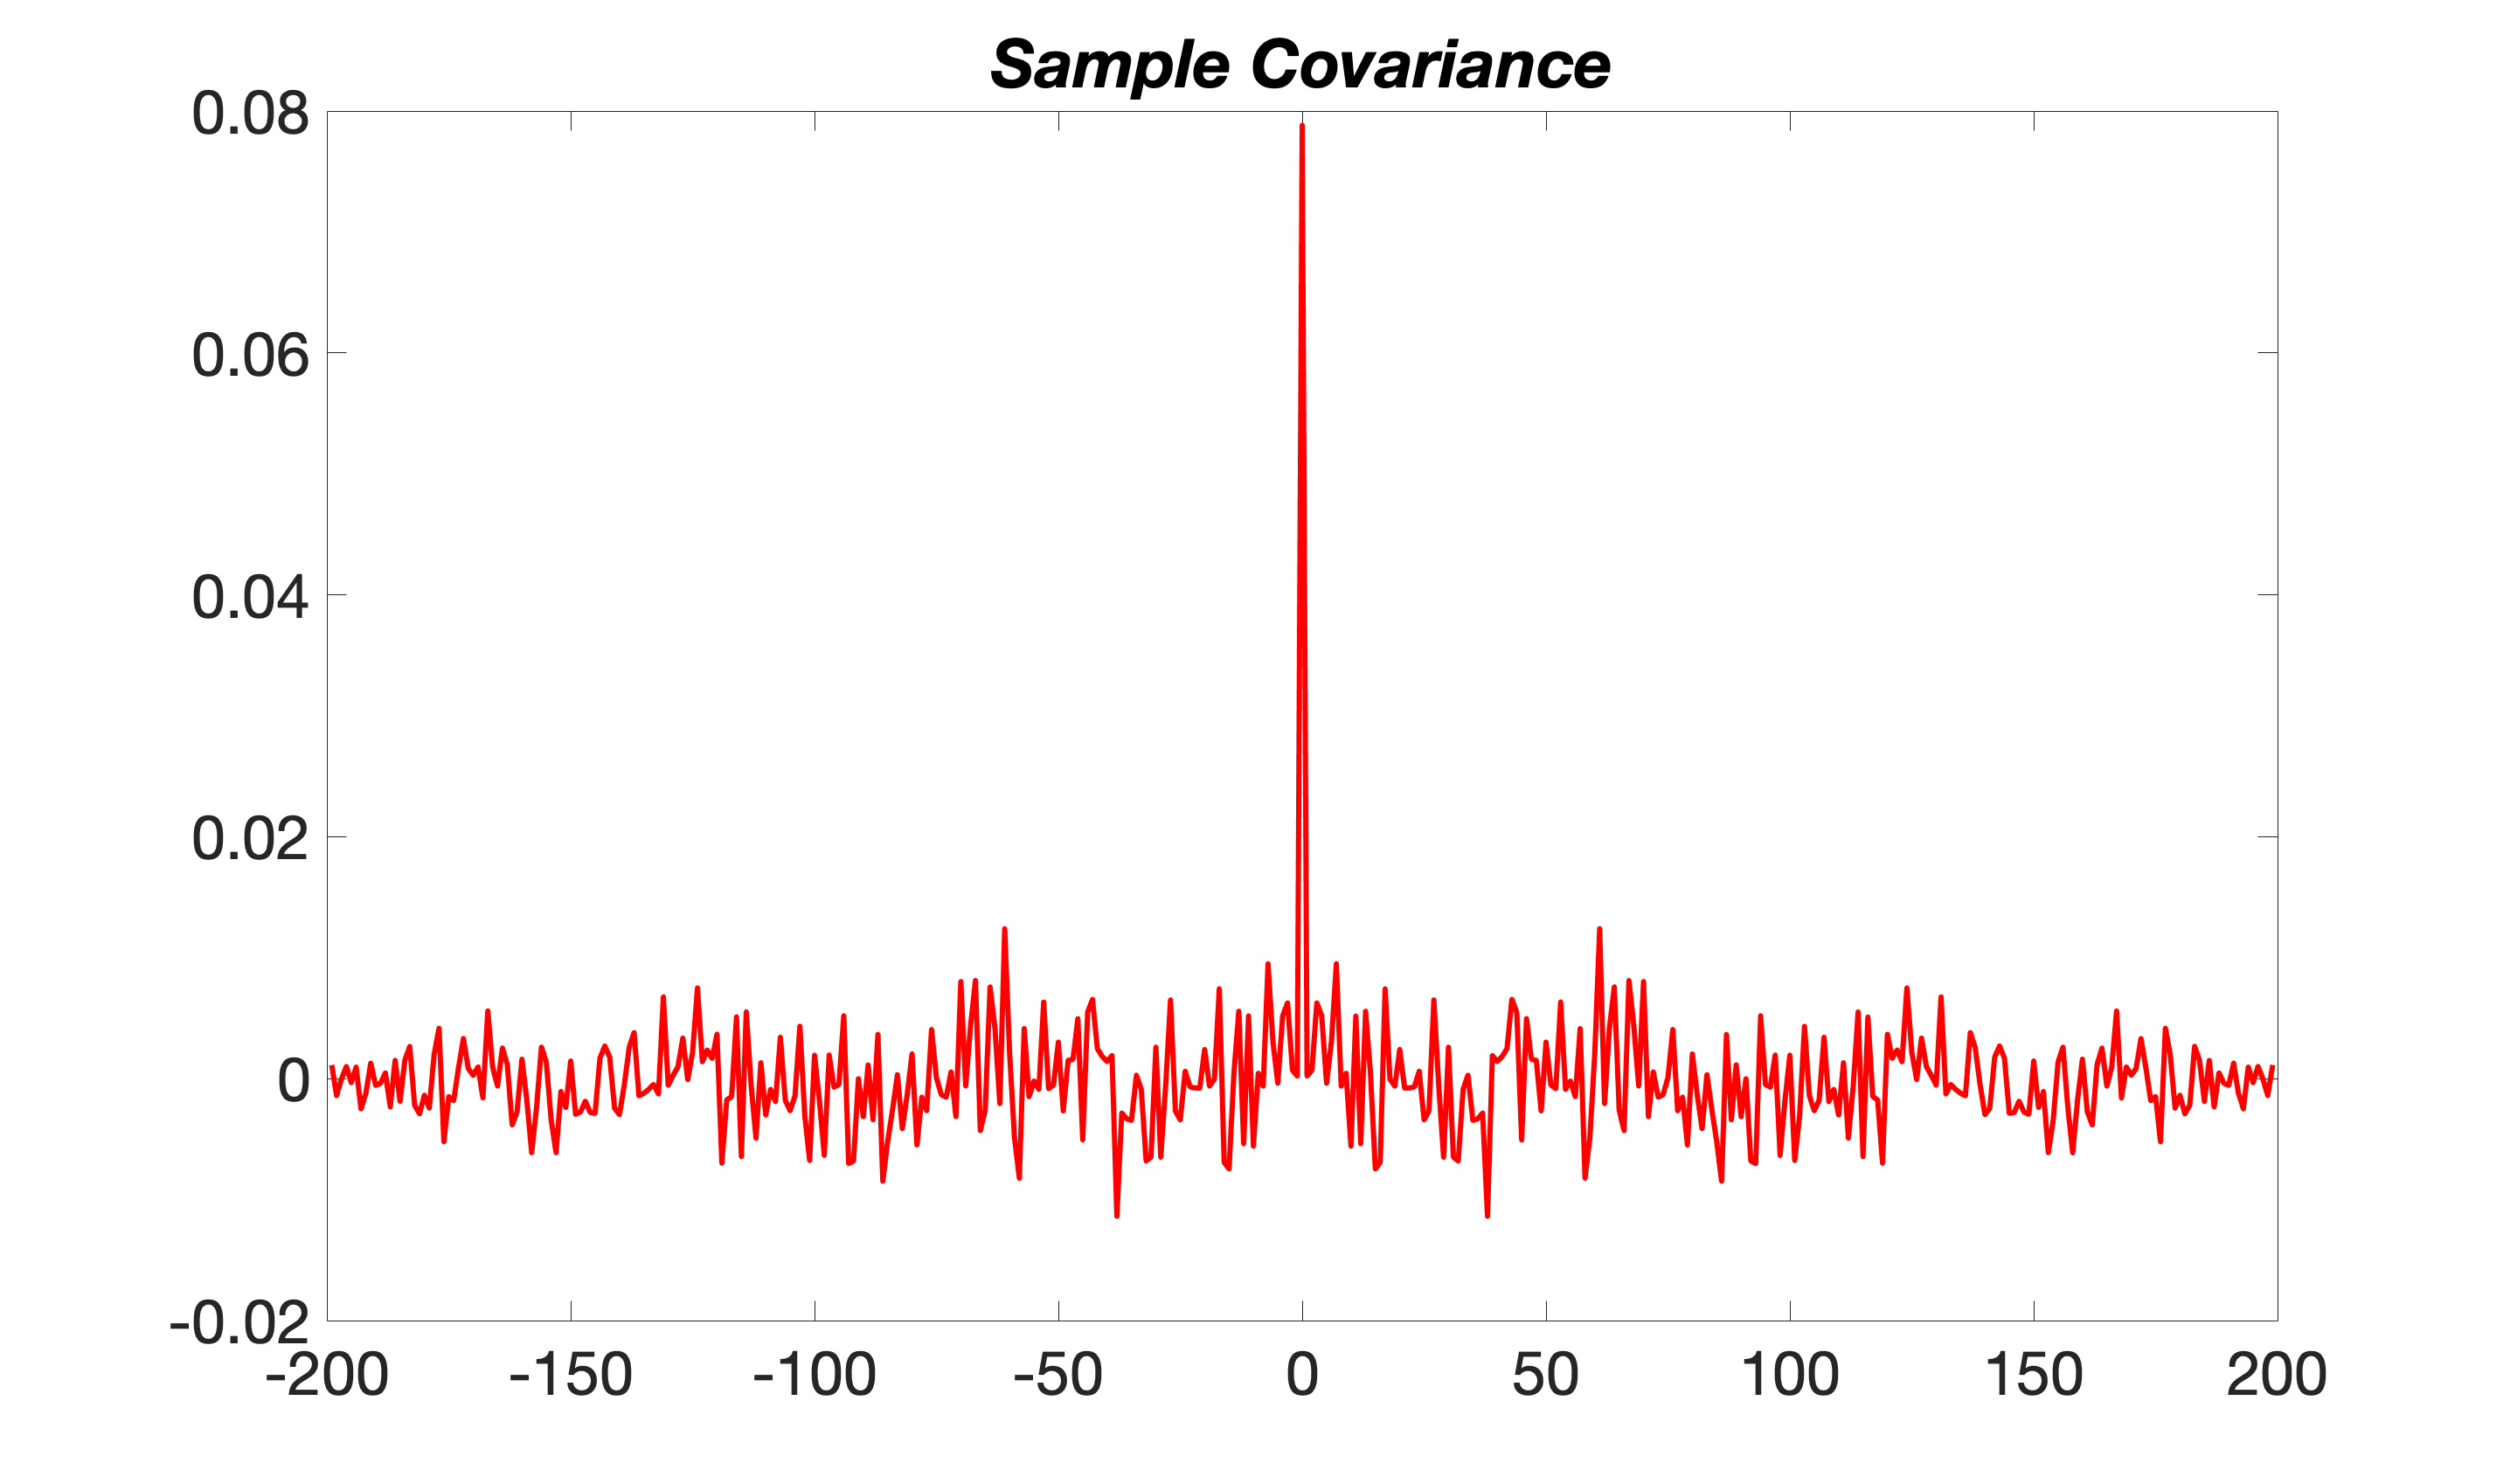
\includegraphics[width=8cm]{ass1_1.png}} }
    \qquad
    \subfloat[Biased Covariance]{ {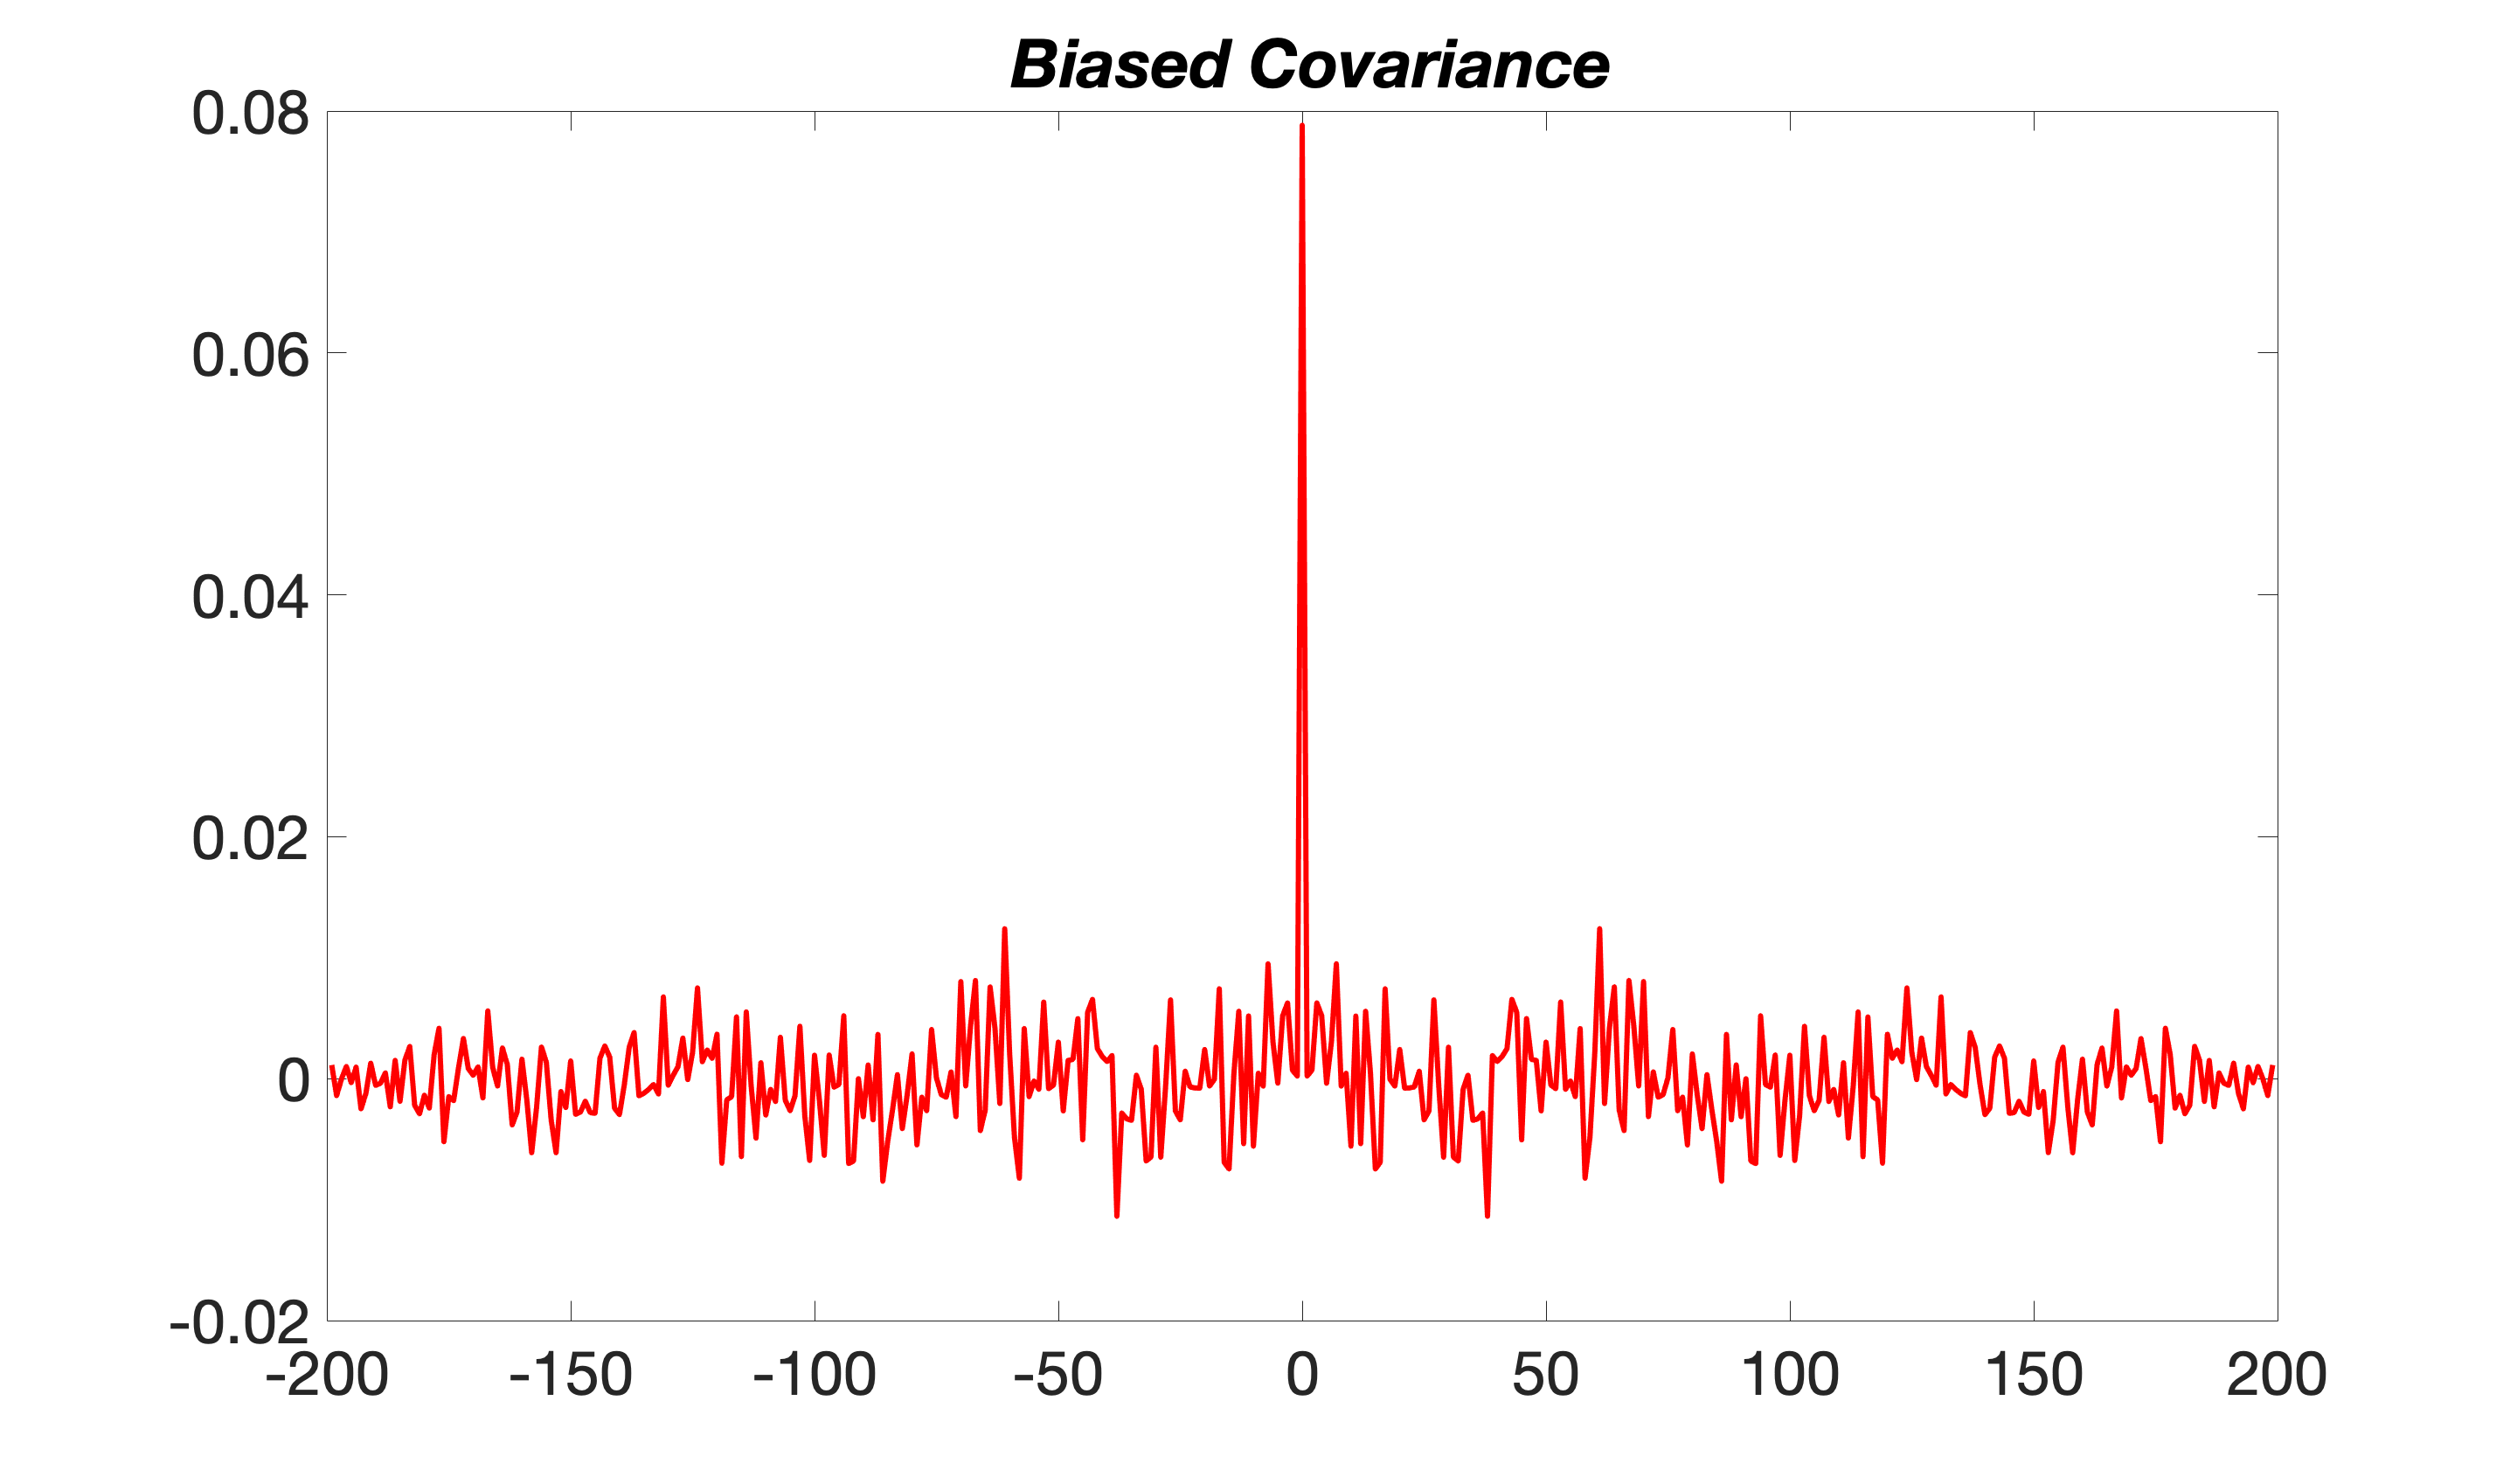
\includegraphics[width=8cm]{ass1_3.png} }}
   % \label{Covariances found using functions \texttt{covfct} and \texttt{xcov}}
    \caption{Covariances found using functions \texttt{covfct}(Sample) and \texttt{xcov}(Biased)}
\end{figure}
\noindent Similarly Figure 2.2 (a) shows the output by the \texttt{covfct} which Figure 2.1 (b) shows the simulated output of the matlab function \texttt{xcov} with unbiased argument. This means that the mean value is known. The point that there is a peak at the center of this sample covariance function means it shall be white noise in wide
sense stationary, the \texttt{xcov} also shows almost no cross-correlation and peak at the center with symmetry at both sides.
\begin{figure}[H]
    \centering
   \subfloat[Modified Sample Covariance]{ {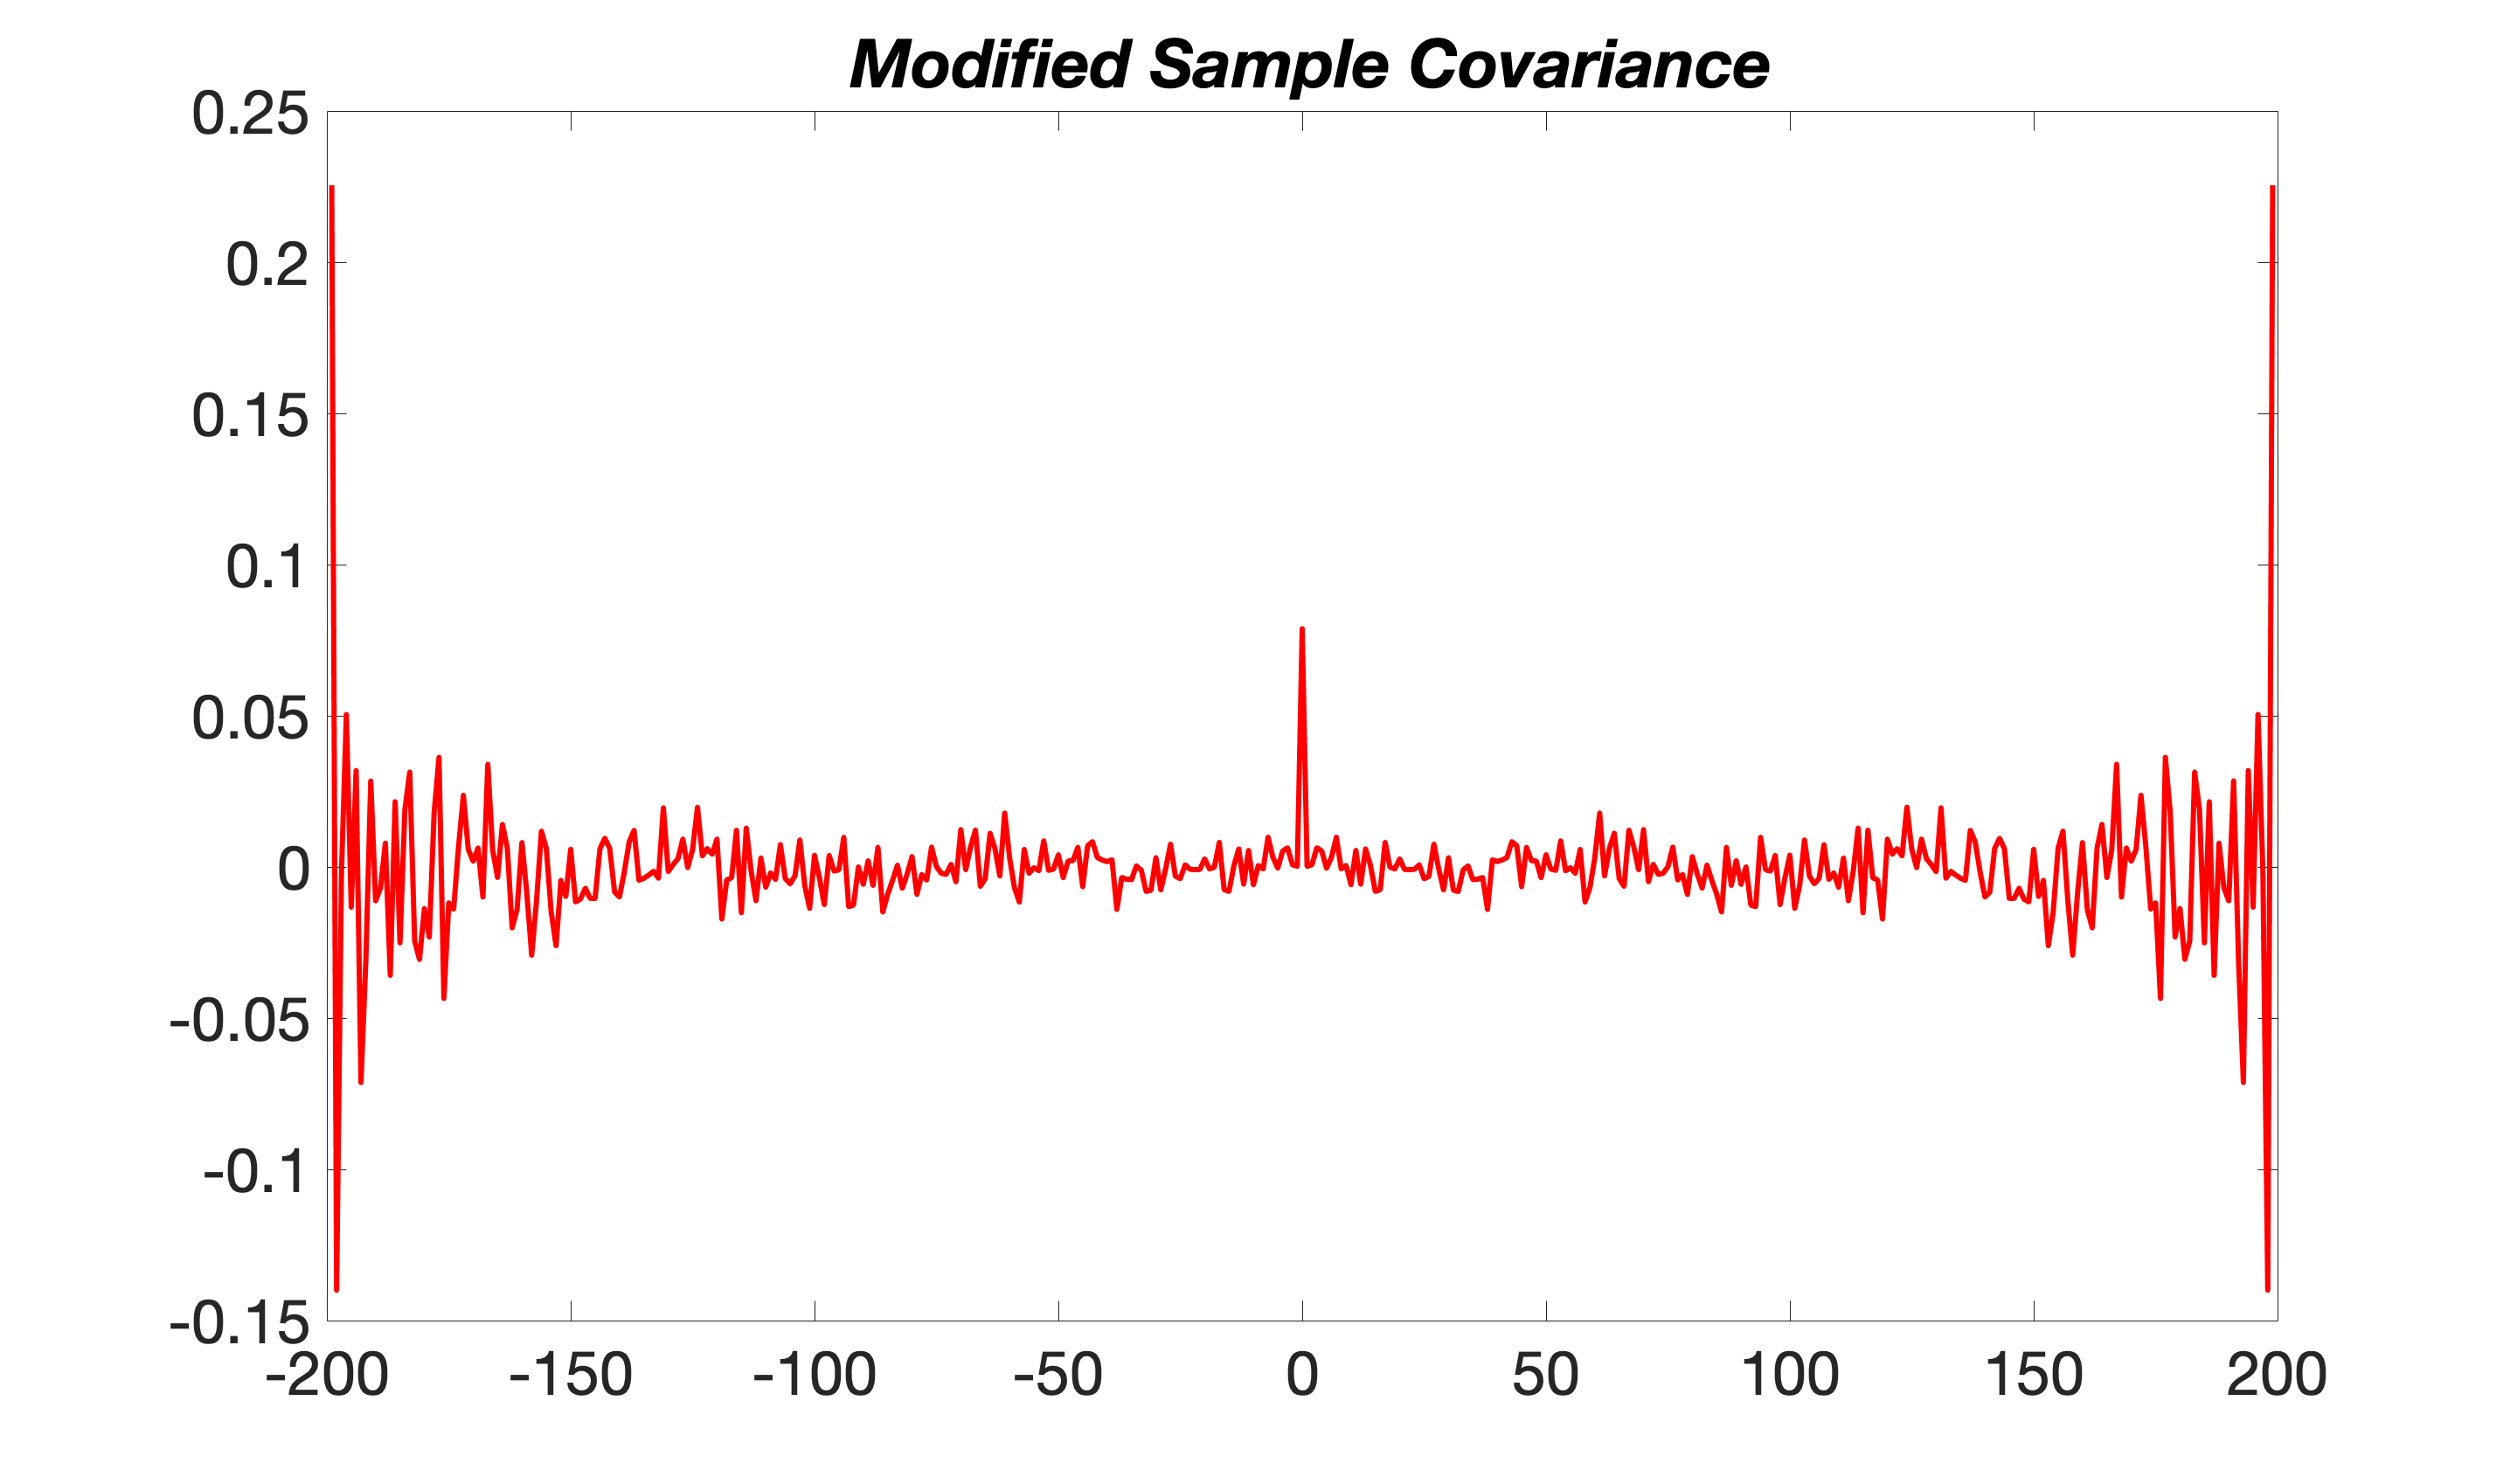
\includegraphics[width=8cm]{ass1_2.png}} }
    \qquad
    \subfloat[Unbiased Covariance]{ {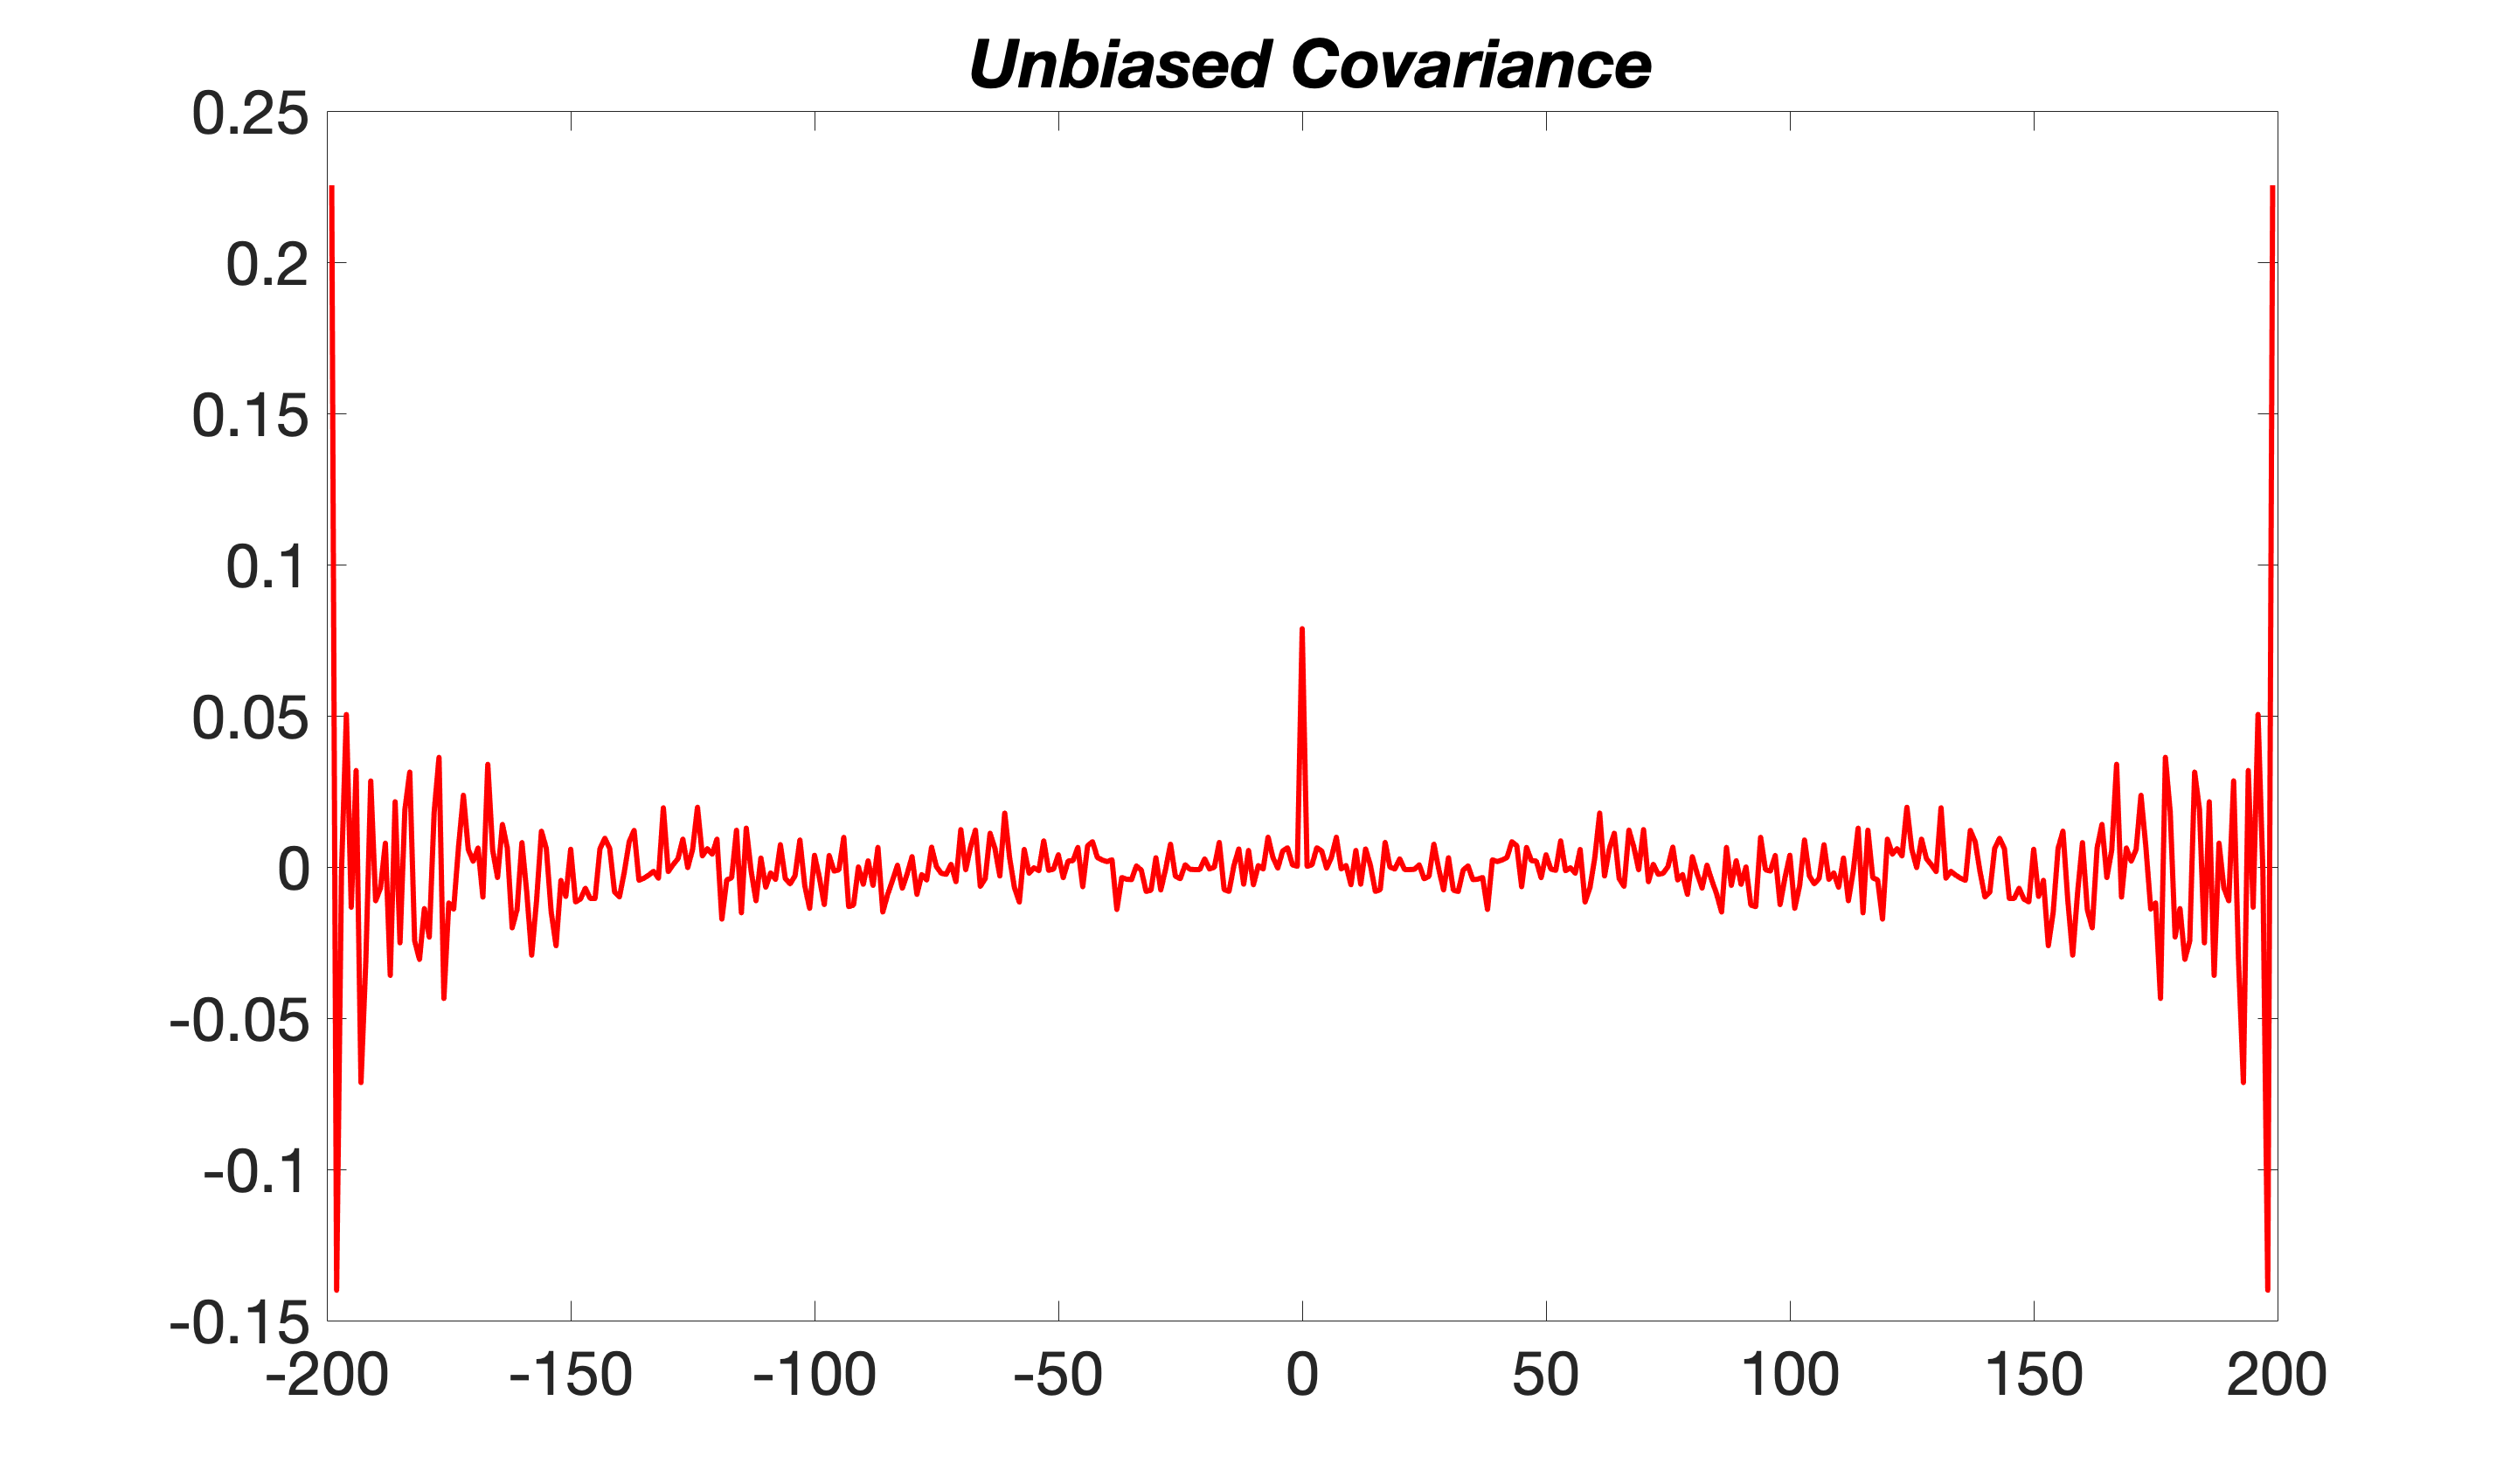
\includegraphics[width=8cm]{ass1_4.png} }}
    \caption{Covariances found using functions \texttt{covfct}(Modified Sample) and \texttt{xcov}(Unbiased)}
\end{figure}
\noindent If one covariance function is plot on x-axis and the other is plot on y-axis, it would be clear that they are equal which is shown in Figure 2.3. It can be concluded that all the outputs are symmetric.
\begin{figure}[H]
    \centering
   \subfloat[Uniform distribution]{ {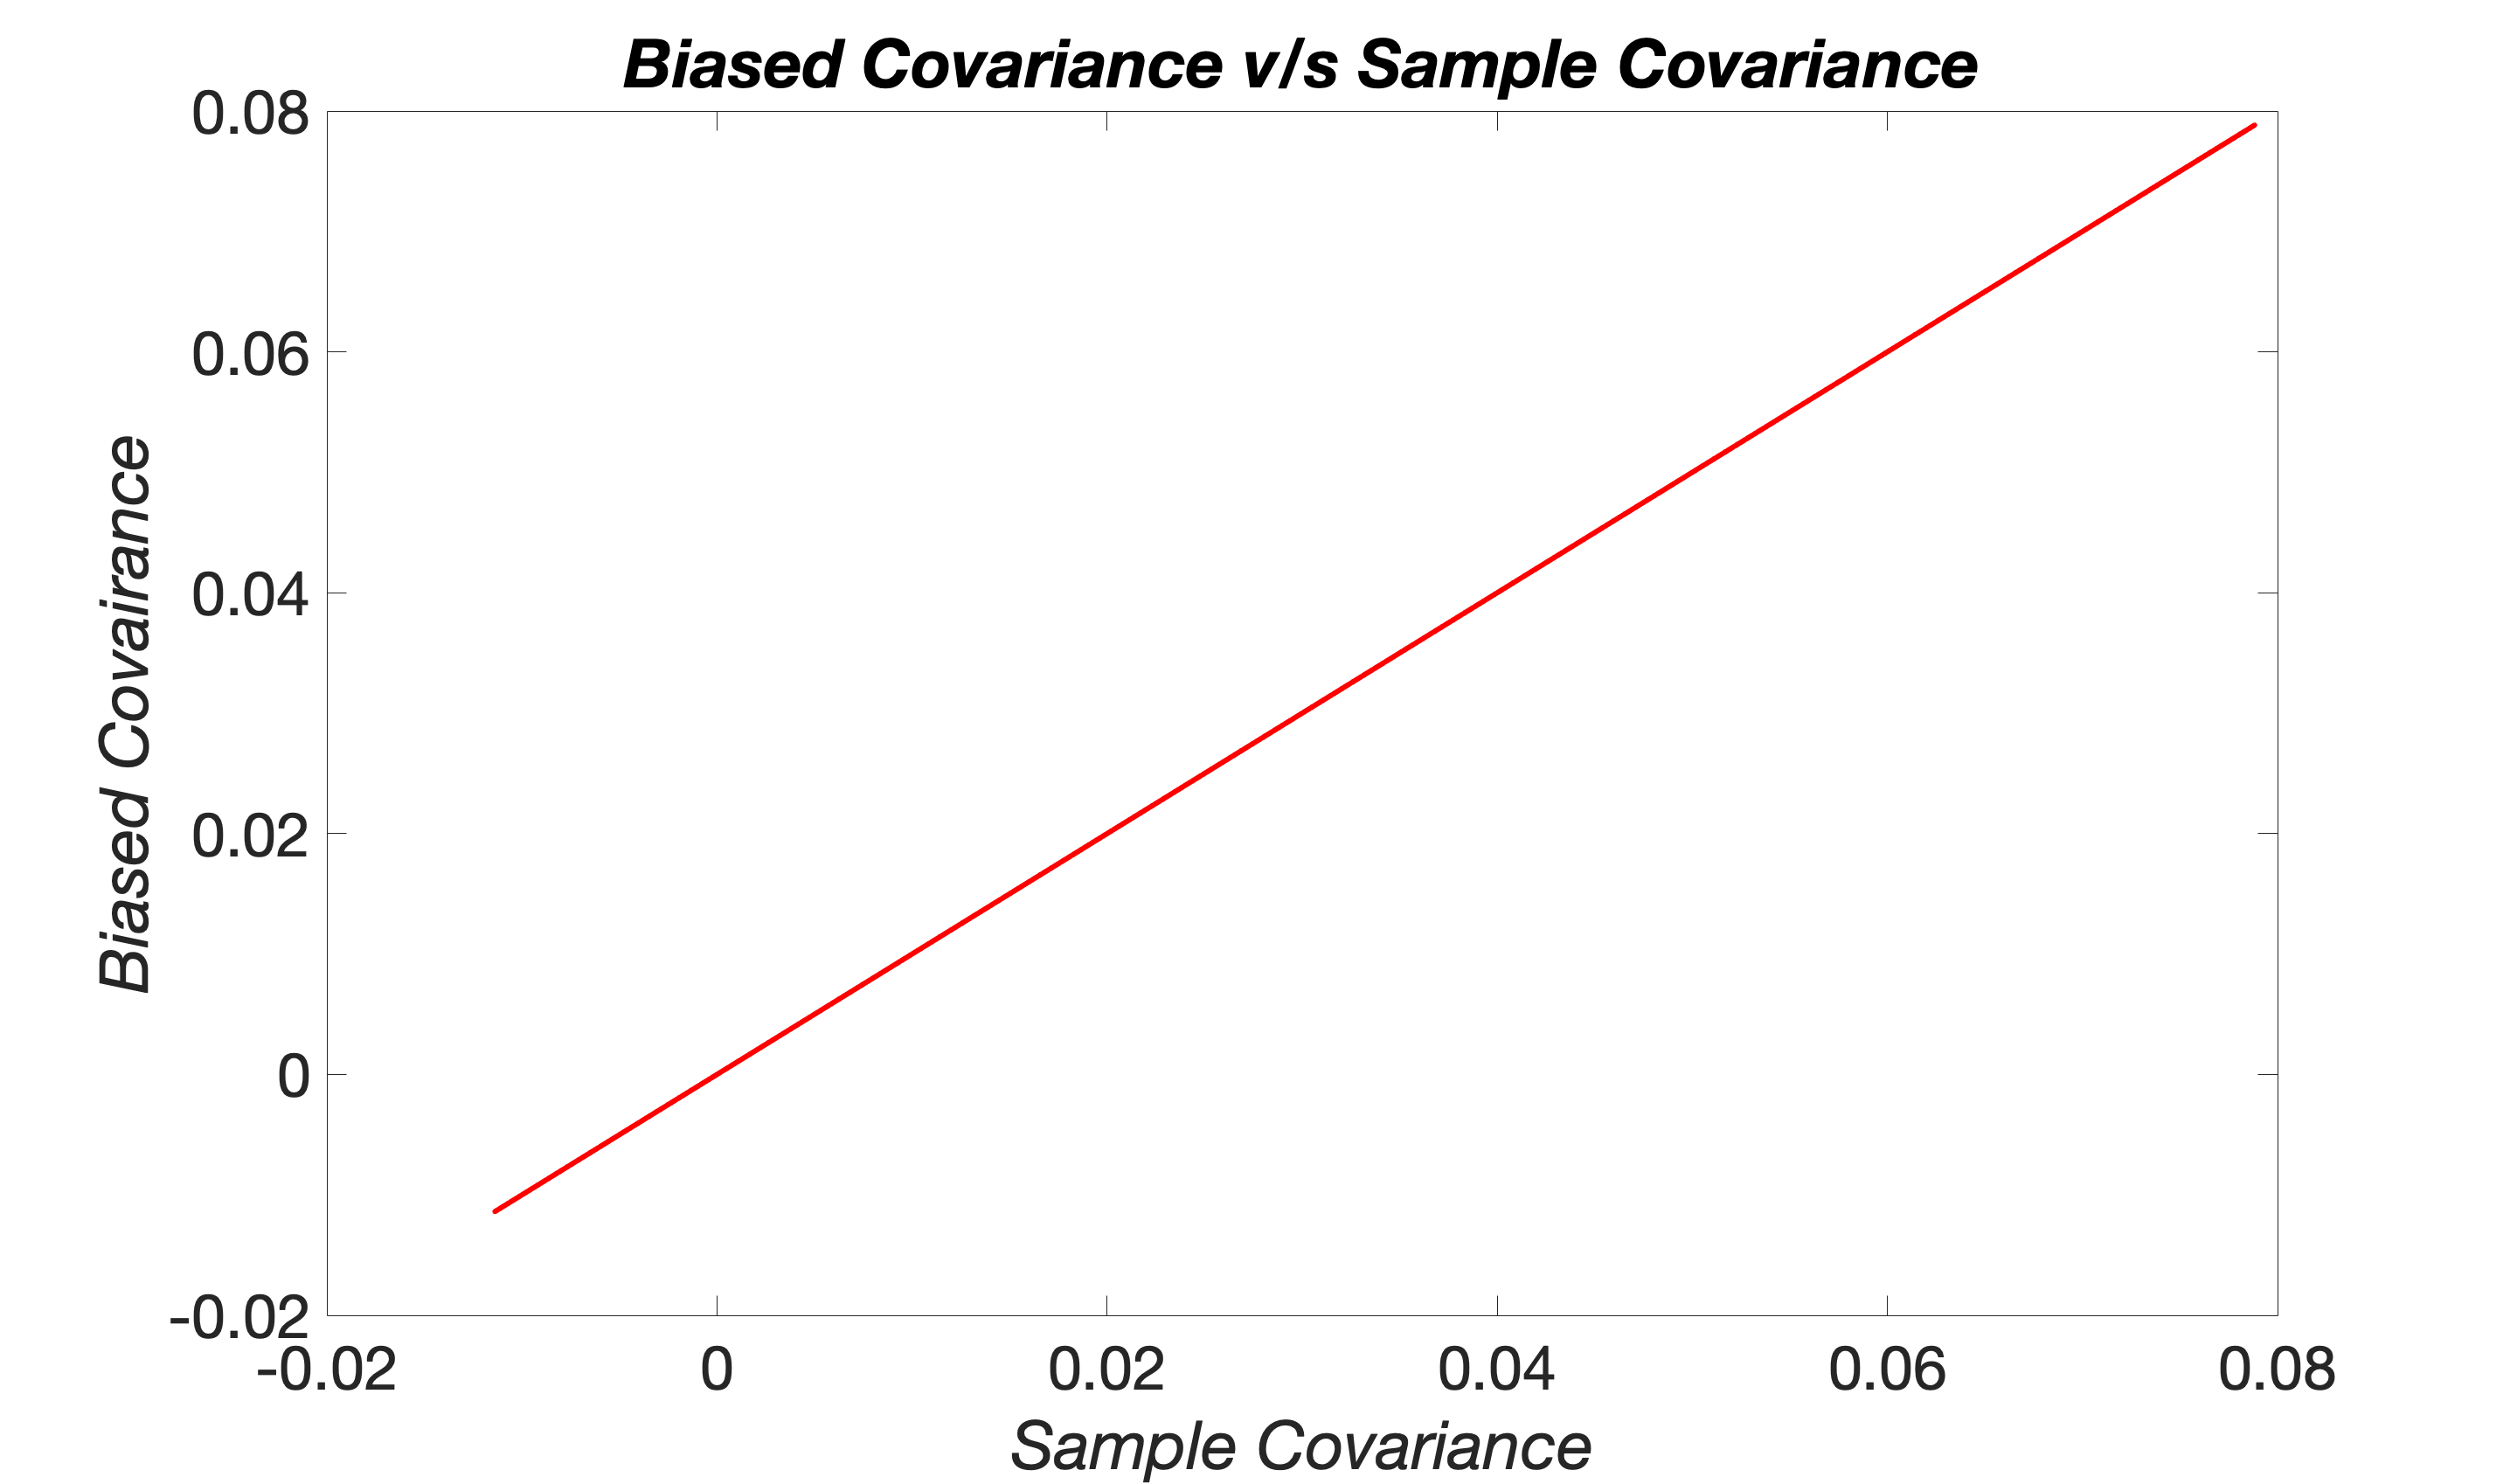
\includegraphics[width=8cm]{ass1_5.png}} }
    \qquad
    \subfloat[Standard normal distribution]{ {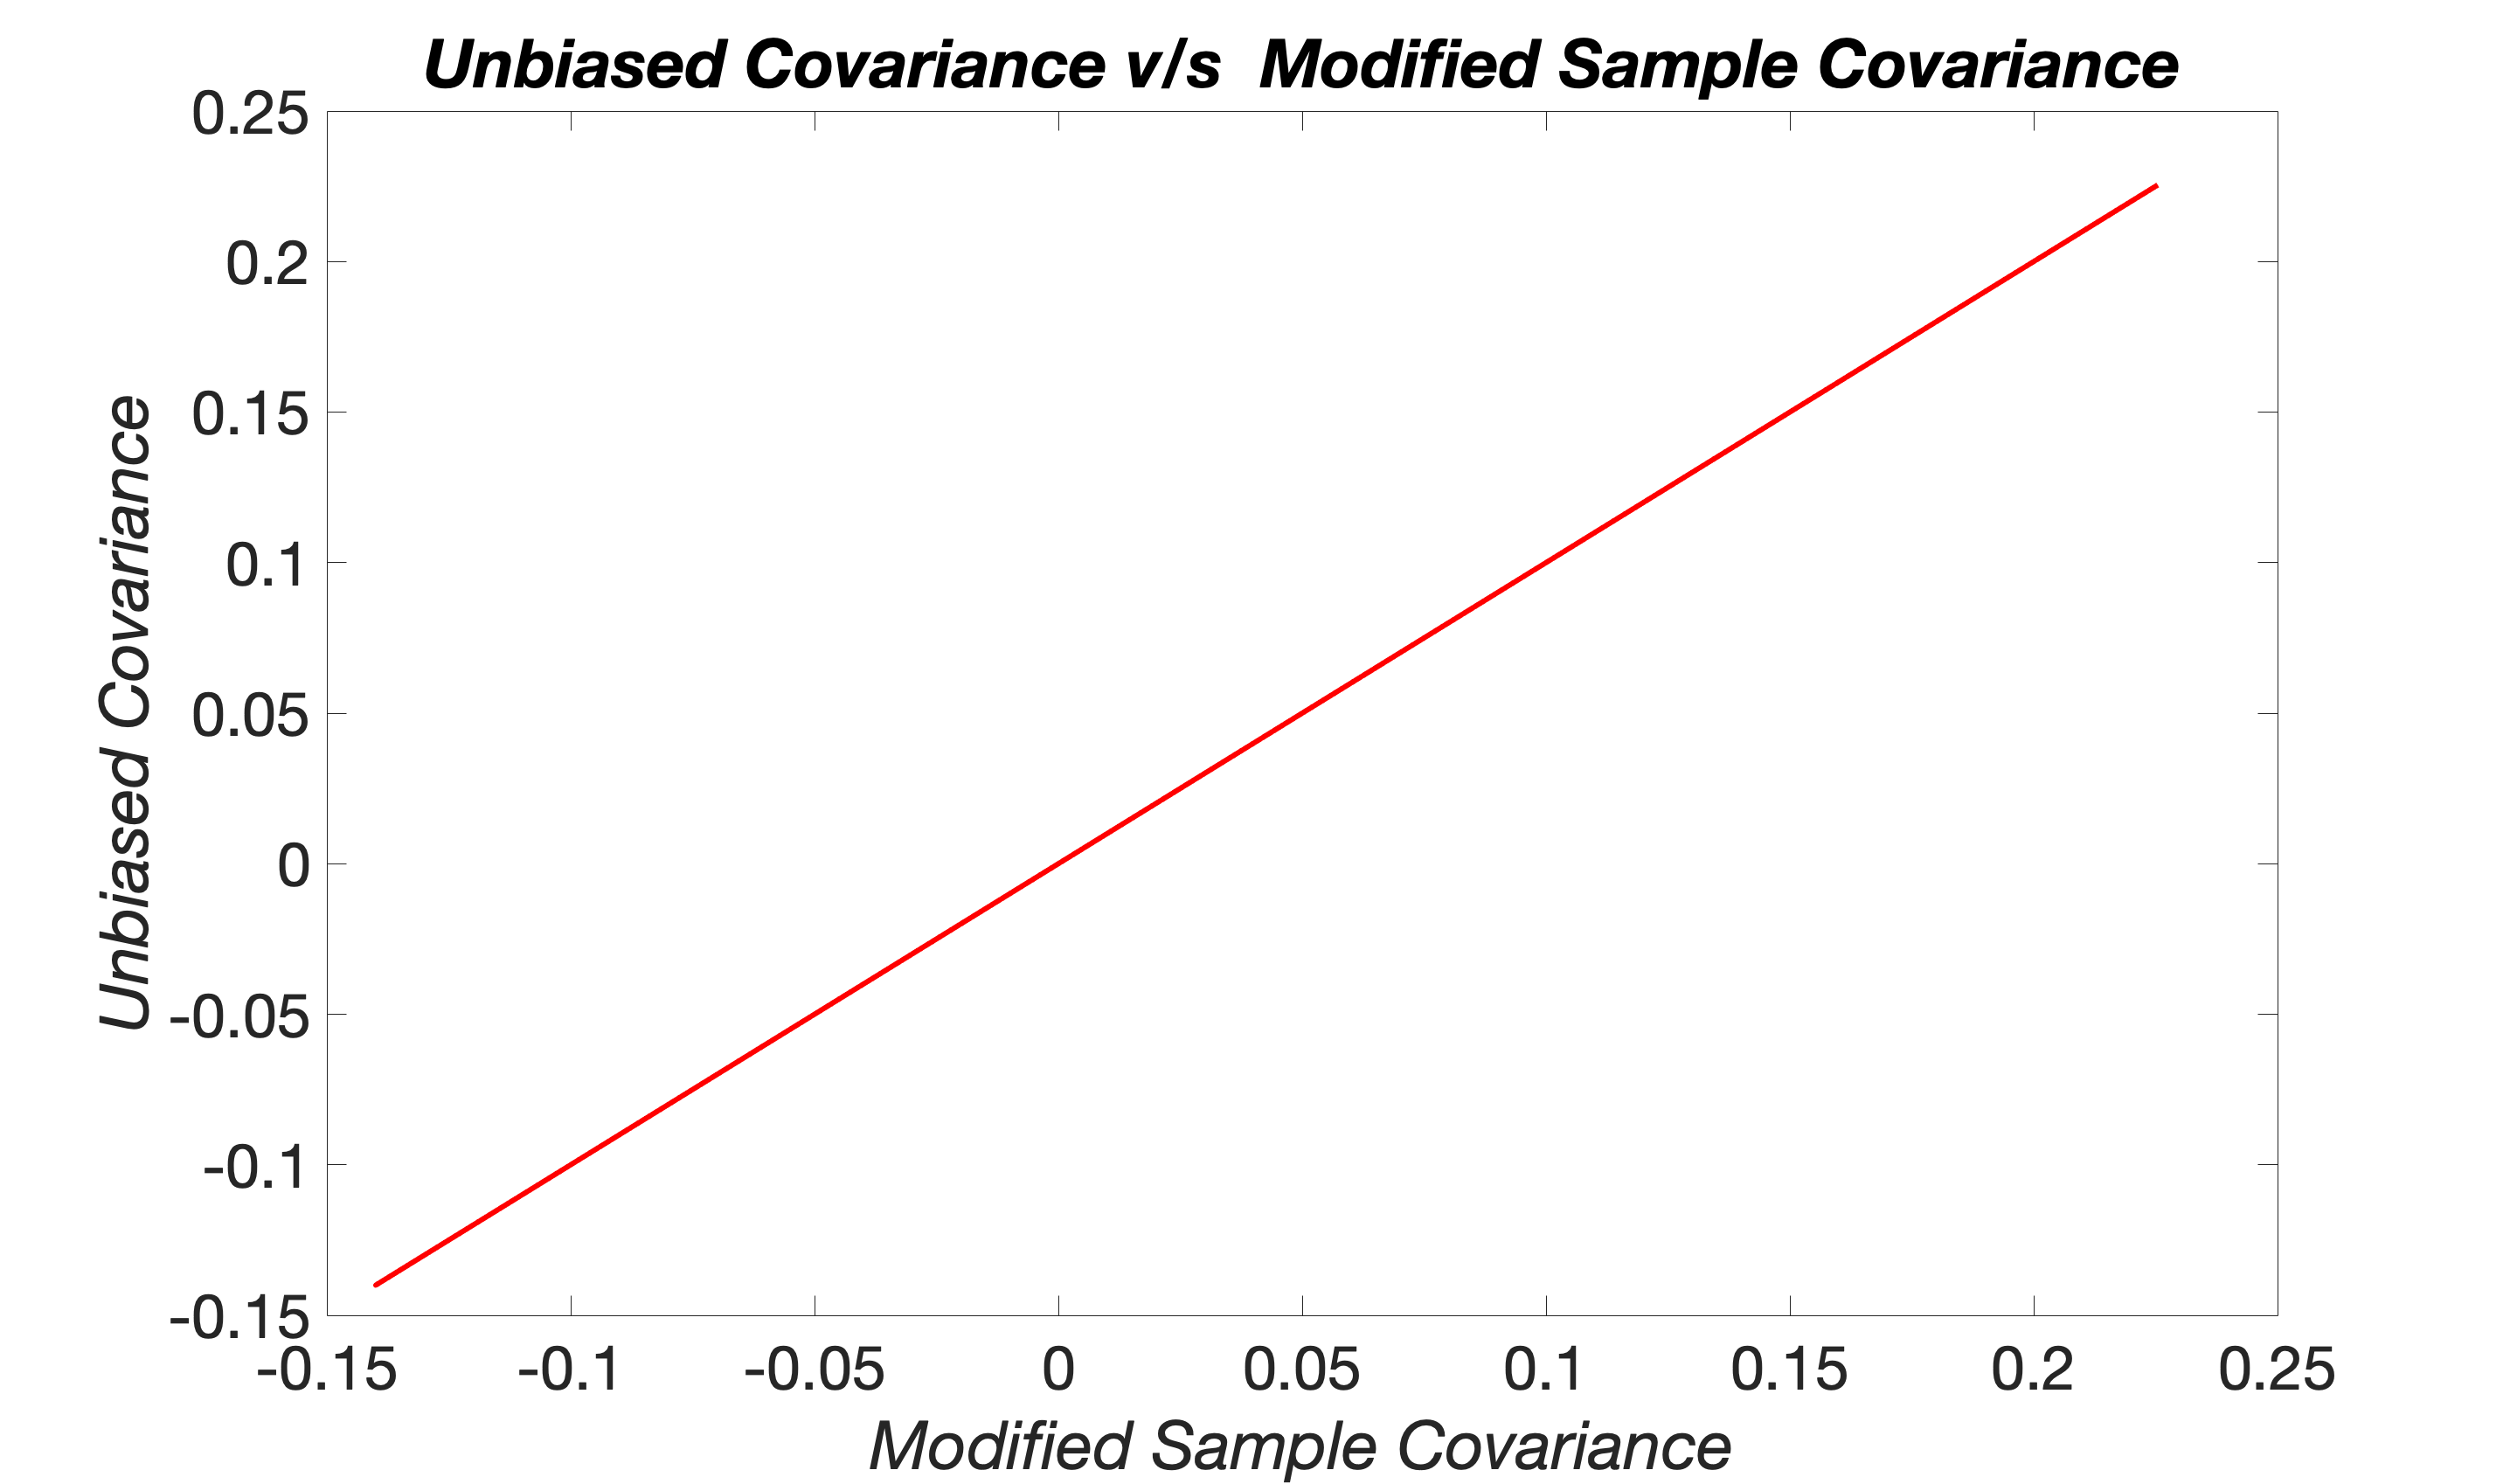
\includegraphics[width=8cm]{ass1_6.png} }}
   \caption{Comparison of the covariances}
   \end{figure}
\noindent \textbf{Inference:} The results obtained by the Matlab function \texttt{xcov biased} match the results of the sample covariance function, and the results of \texttt{xcov unbiased} match the results of the modified sample
covariance function. The sample covariance function is more accurate in case of a large number of observations because the variance converges to zero when the number of observations is getting very large. However, the modified sample variance function gives better results when the number of observations is limited.


%%%%%%%%%%% code 2 %%%%%
\section{ Generation of AR($p$) - processes} 
\noindent \textbf{Task:} Load \texttt{dat1\_2} that includes a realization of white noise. For the generation of an AR($p$) process you have to filter the white noise by a recursive filter with the filter coefficients $a_1 = 0.5, a_2 = 0.3, a_3 = 0.1, a_4 = 0.7, a_5 = 0.3.$ Use the MATLAB-function \texttt{filter}. Save the white noise and the AR ($\rho$) - process for later use in \texttt{dat4\_1}.
 \\

\noindent \textbf{Solution:}
\noindent The data which includes a realization of white noise is loaded at first. This white noise is filtered using the recursive filter with the filter coefficients $a_1 = 0.5, a_2 = 0.3, a_3 = 0.1, a_4 = 0.7, a_5 = 0.3.$We used the MATLAB function \texttt{filter} for this process and both white noise as well as AR($\rho$) - processes is saved in \texttt{dat4\_1}

\noindent \textbf{MATLAB code:}
\lstinputlisting{assignment4_2.m}

\noindent \textbf{Output:}
\noindent Figure 2.4 shows the impulse response of the filter.

\begin{figure}[H]
\centering
{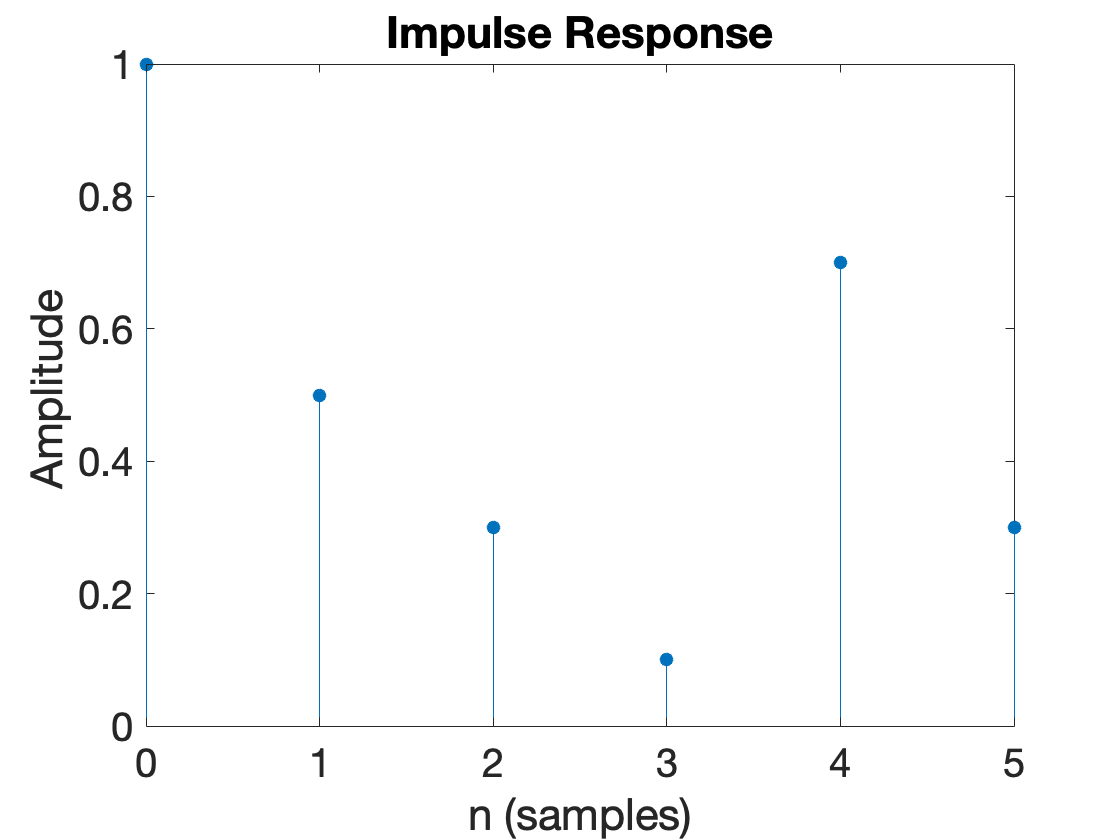
\includegraphics[scale=0.25]{ass2_1.png}}
\caption{Impulse response of the filter }
\end{figure}

\noindent \textbf{Inference:} The Auto-Regression process is been realized by the filtering the normally distributed random numbers using the Matlab function filter, with the given coefficients: a = [1,0.5,0.3,0.1,0.7,0.3], b = [1]. The mean value of the impulse response is zero.  After obtaining the coefficients the AR($p$)-process is being generated, and the data are saved for further processing.

%%%%%%%%%%%%%%% code 3 %%%%%
\newpage

\section{ LS-Estimation } \label{ LS-Estimation  }
\noindent \textbf{Task:} Carry out a LS - Estimation of the parameters $a_i(i=1,2,...,5)$ and the variance ${\sigma_Z}^2$of the AR($p$)-process.

\noindent \textbf{Solution:}  
\noindent The LS - Estimation of the parameters $a_i(i=1,2,...,5)$ and the variance ${\sigma_Z}^2$of the AR($p$)-process is carried out by the following code.

\noindent \textbf{MATLAB code:}
\lstinputlisting{assignment4_3.m}

\noindent \textbf{Output:}
\noindent The output after execution of the code is shown below. 
\begin{figure}[H]
\centering
{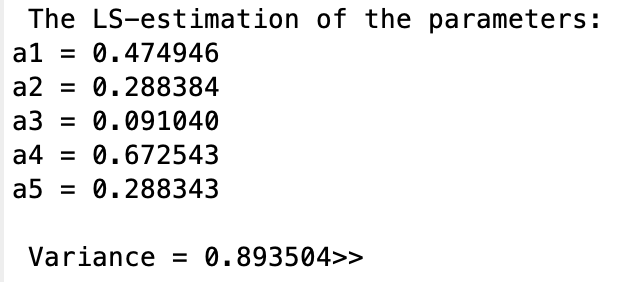
\includegraphics[scale=1.15]{ass3_1.png}}
\end{figure}

\noindent \textbf{Inference:} The parameters and the variance is calculated and shown above.

%%%%%%%% code 4 %%%%%


\section{ Empiric Yule-Walker-Equation  } \label{ Empiric Yule-Walker-Equation l}
\noindent \textbf{Task:}Determine the first 11 values of the sample covariance function, e.g.  $\hat{c}_{xx}(0),...\hat{c}_{xx}(10)$ using function \texttt{covfct}. Estimate the parameters $a_1(i=1,2,...,5)$ and ${\sigma_z}^2$ by solving the empirical Yule-Walker-Equation via the Gaussian elimination algorithm. (Note: Use the MATLAB-function \texttt{toeplitz} to generate the coefficient matrix and read the MATLAB-help for the operator \texttt{backslash}.)

\noindent \textbf{Solution:} The MATLAB-function \texttt{toeplitz} is used to generate the coefficient matrix. The estimation of the first 11 values of the sample covariance function is carried out by the following code.

\noindent \textbf{MATLAB code:}
\lstinputlisting{assignment4_4.m}
\noindent \textbf{Output:} Applying \texttt{covfct} function to the AR($p$)-process, the sample covariance function is obtained and the first 11 values are listed in Fig 2.5. The coefficient matrix, estimated parameters as well as the variance is the output of the MATLAB code. 
\begin{figure}[H]
\centering
{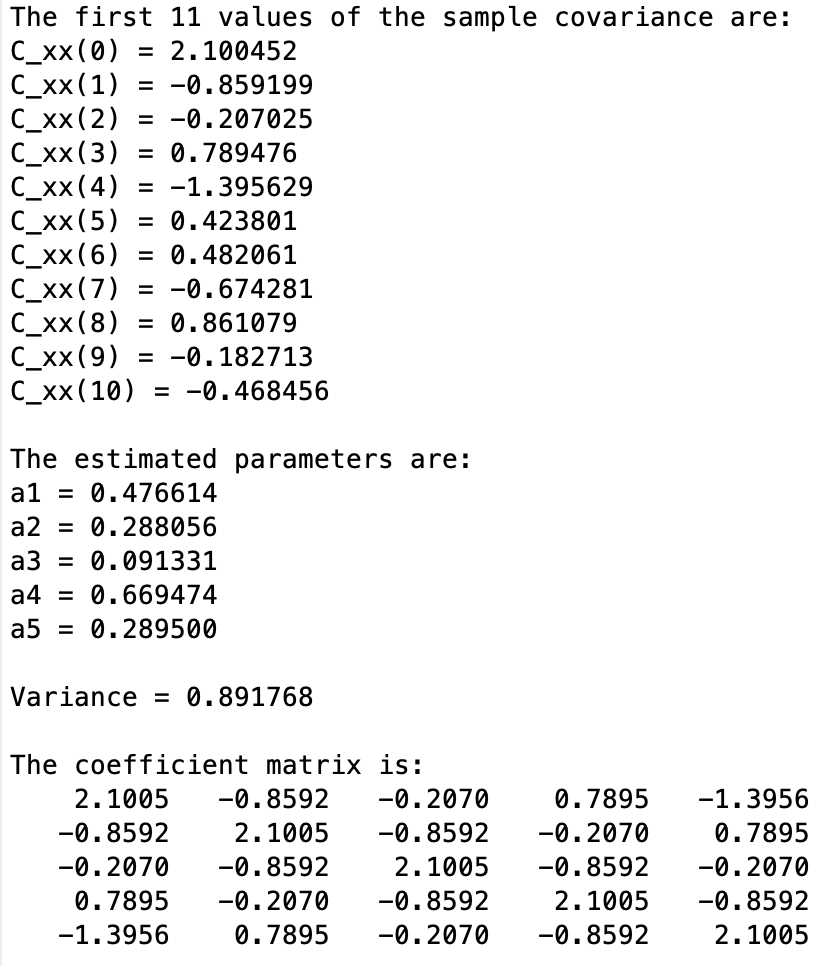
\includegraphics[scale=0.66]{ass4_1.png}}
\end{figure}

\noindent \textbf{Inference:} The parameters and the variance is calculated and shown above.

%%%%%%%%%%%  code 5  %%%%%

\section{Levinson-Durbin-Algorithm}  \label{Levinson-Durbin-Algorithm }
\noindent \textbf{Task:} Write a function \texttt{levindur} for implementation of the Levinson-Durbin-Algorithm. Estimate with this function and the sample covariance function \texttt{covfct} the parameters $a_1(i=1,2,...,5)$ and the variance ${\sigma_z}^2$.
 
 \noindent \textbf{Solution:} A function \texttt{levindur} is written using the Matlab function Levinson for the implementation of the Levinson-Durbin-Algorithm.
 
 \noindent \textbf{MATLAB code:}
\lstinputlisting{assignment4_5.m}

 \noindent \textbf{Output:}
 \noindent Again the parameters $a_i(i=1,2,...,5)$ and ${\sigma_Z}^2$ are estimated and the results are given as follows.
\begin{figure}[H]
\centering
{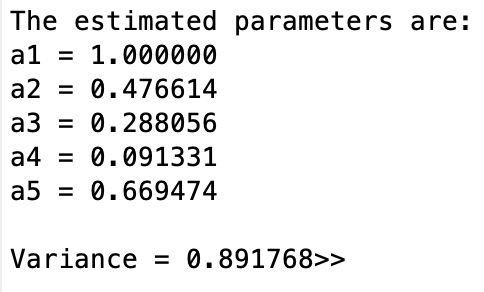
\includegraphics[scale=0.65]{ass5_1.png}}
\end{figure}

\noindent \textbf{Inference:} We can infer that the the values are similar as obtained by solving empirical-Walker-Equation.
%%%%%% code 6 %%%%%%

\section{ Estimation of the model order  }  \label{ Estimation of the model order }
\noindent \textbf{Task:} Estimate the parameters $a_1(i=1,2,...,5)$ and ${\sigma_z}^2$ as in section 4.2.5, but now for the wrong model order $p = 4$ and $p = 6.$ Compare the estimated parameters with those obtained in section 4.2.5. Which consequences have an underestimation or an overestimation of the model order? Estimate
now for the model order $k(k=1,2,...,10)$ and the variance ${\sigma_{Z,k}}^2$ with the Levinson-Durbin-Algorithm.
Present the result in a diagram. Draw also the values of the Akaike and Rissanen criterion and deduce from them the model order $p$ of the AR($p$)-process. 



\noindent \textbf{Solution:} The parameters $a_i(i = 1, 2,...,5)$ and ${\sigma_Z}^2$ are estimated for two model orders p=4 and p=6 using the code given below.
\noindent \textbf{MATLAB code:}
\lstinputlisting{assignment4_6.m}

\begin{figure}[H]
\centering
{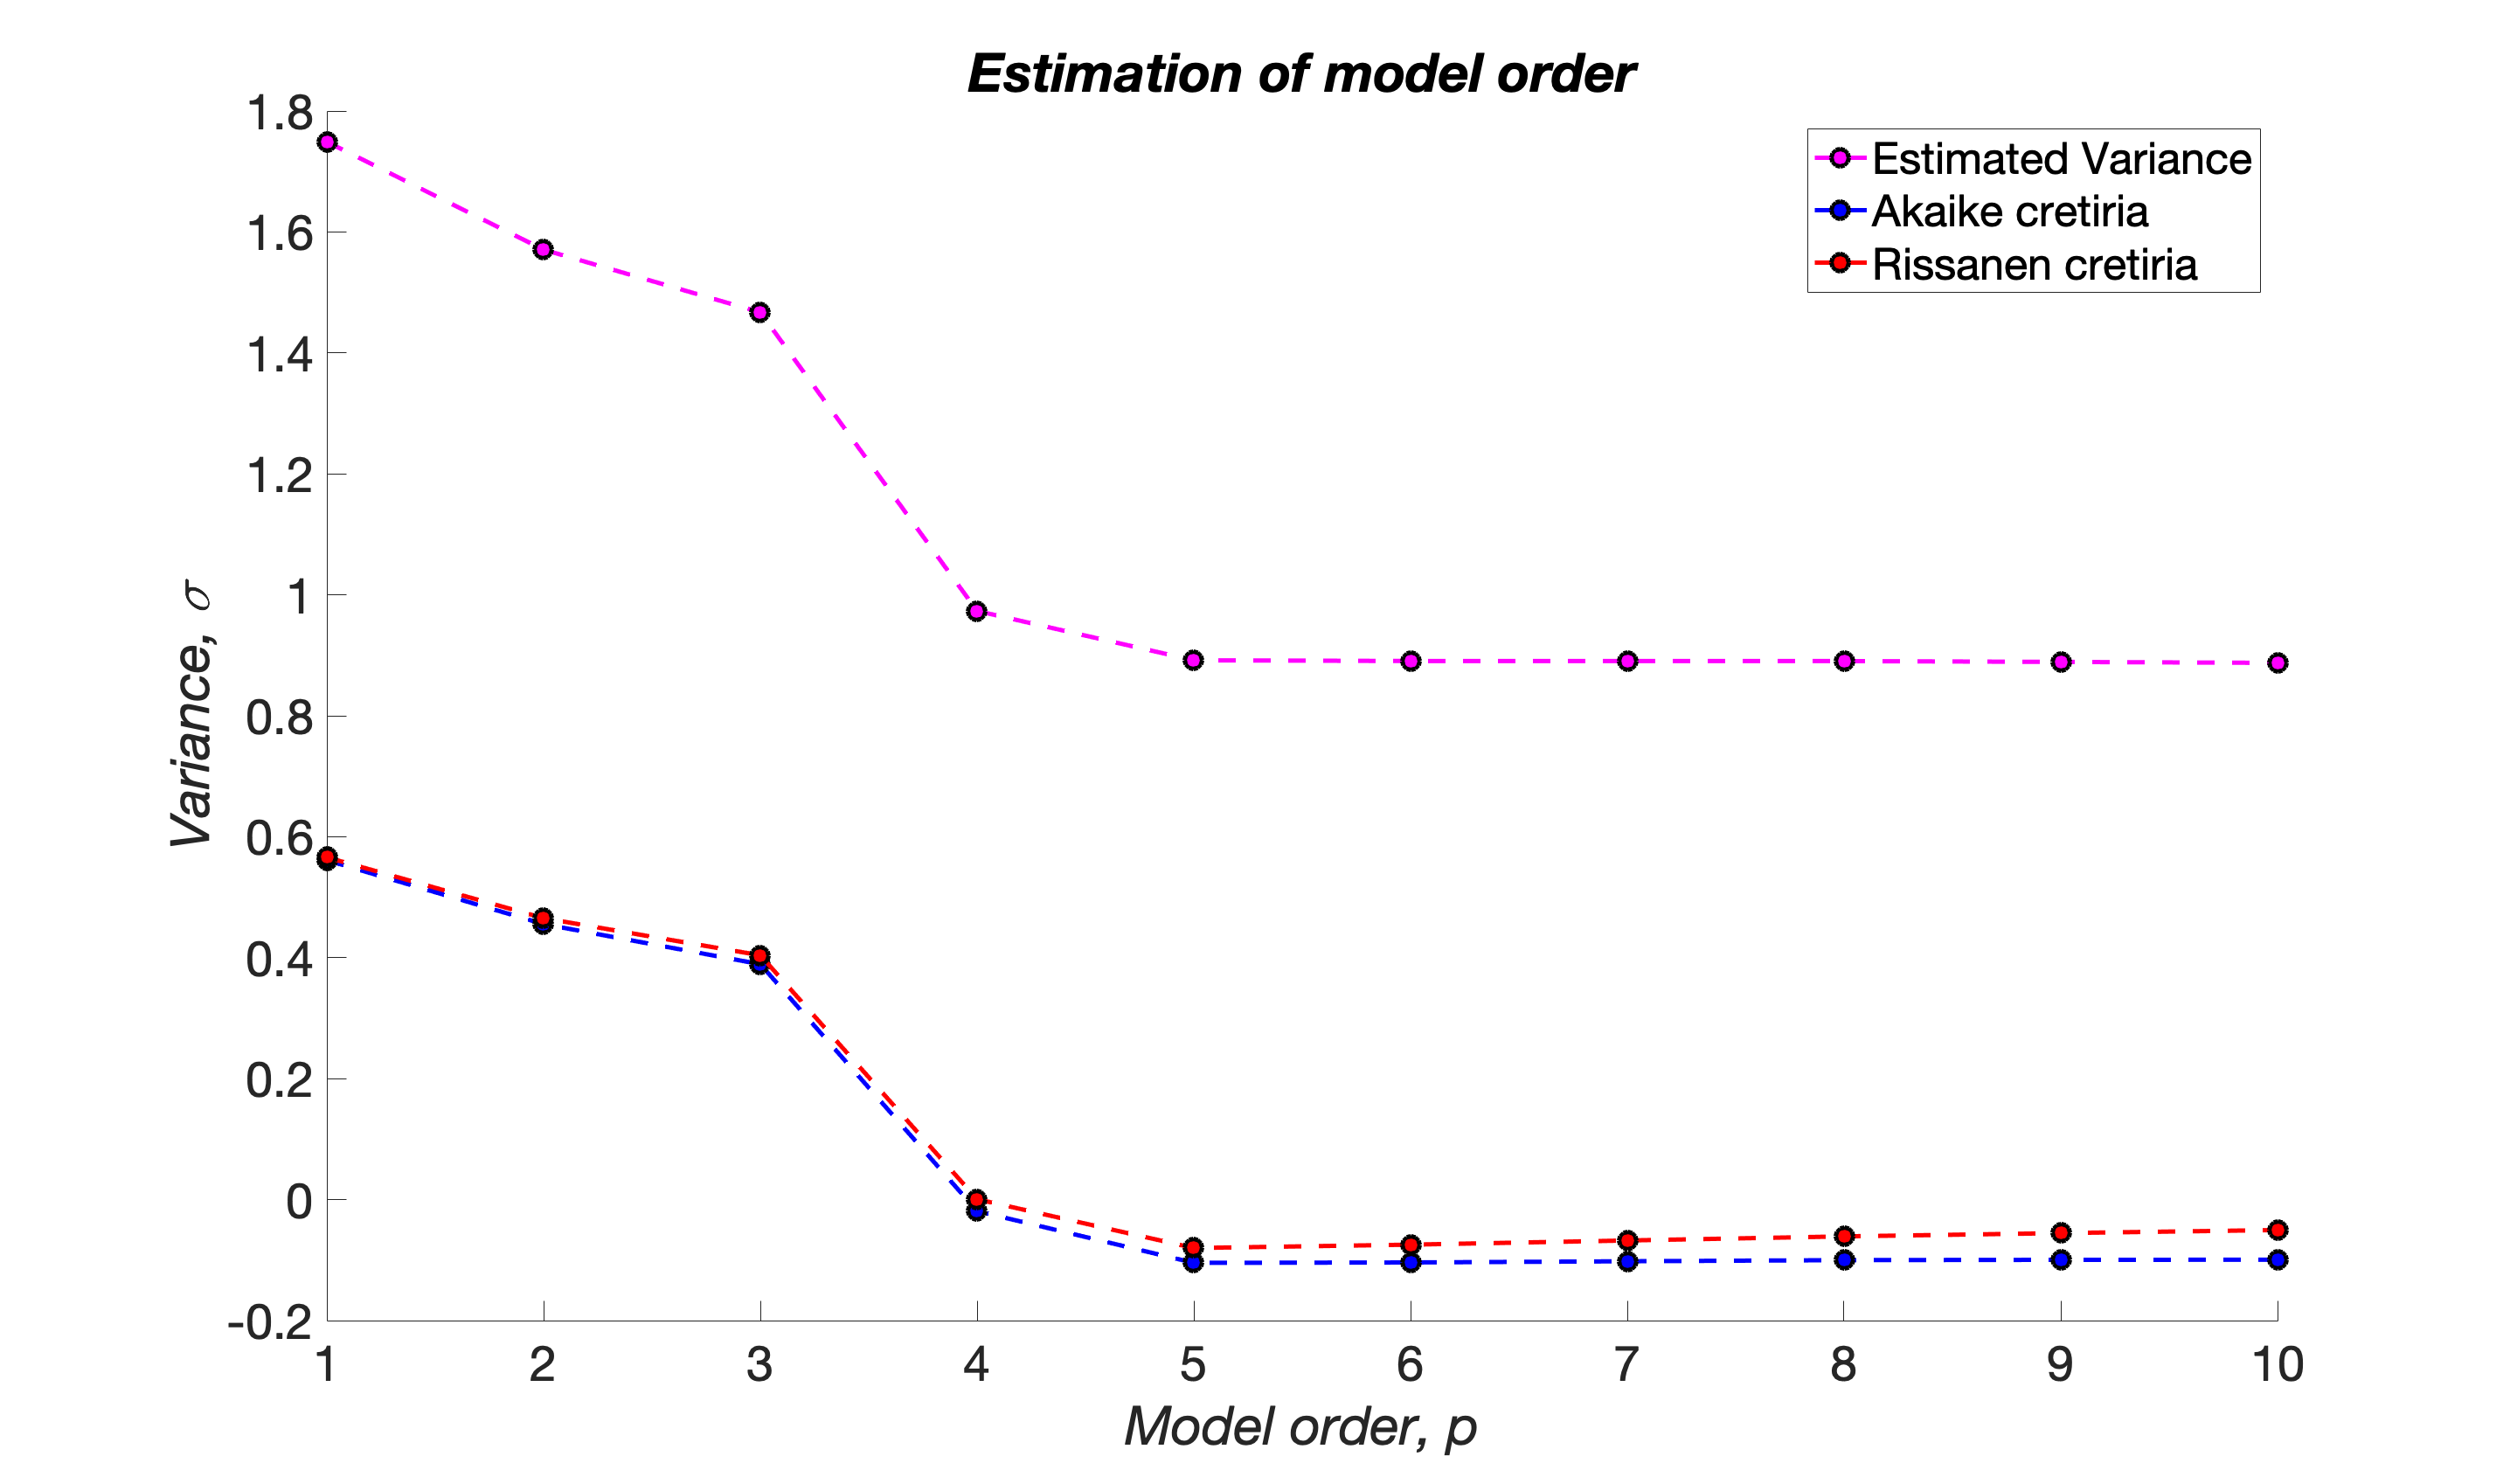
\includegraphics[scale=0.15]{ass6_1.png}}
\caption{Estimation of model order }
\label{Estimation of model order}
\end{figure}

 \noindent \textbf{Output:} 
 \noindent It is evident that for lower order the variance is higher, hence high error. And for higher order it is less. Comparing the resulting parameters for model orders $p=4$ and $p=6$ with the parameters estimated for the order $p=5$, it can be seen that slight differences between the parameters estimated for the order $p=6$ and $P=5.$ Whereas the differences are big between the parameters estimated for the model with order $p=4$ and $p=5.$ So it is better to have an overestimation of the model order than an underestimation, because underestimation will lead to a big error. In order to determine the correct model order, the variance is estimated for the orders from 1 to 10. 

\begin{figure}[H]
\centering
{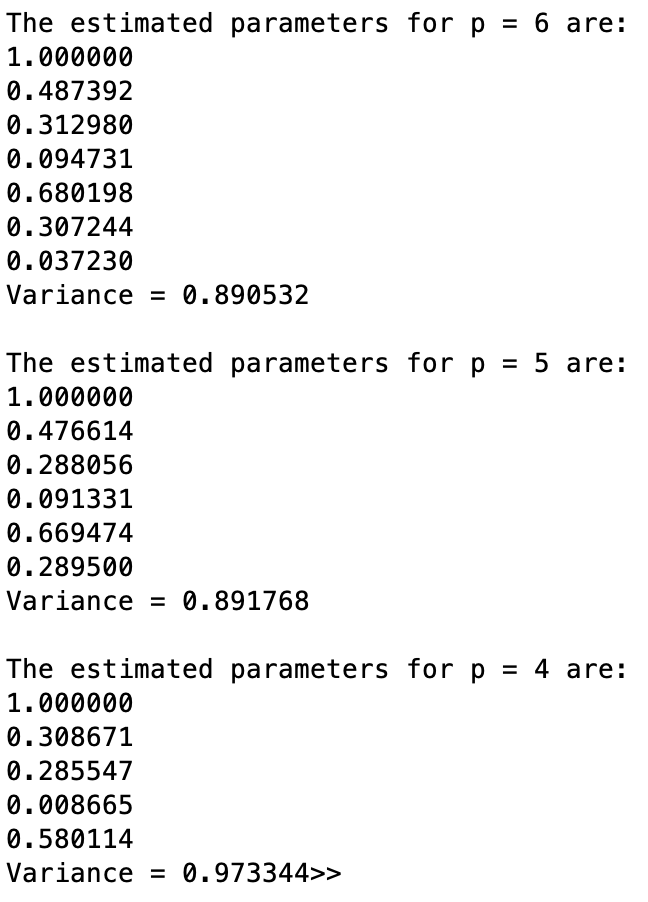
\includegraphics[scale=0.55]{ass6_2.png}}
\end{figure}
\noindent In information theory, the Akaike and Rissanen criterion is considered for computing the statistical quality of data. Here, the variance is measured along with its order. For $p=5,$ the minimum could be achieved for both the model (so this gives confidence). Rissanen (MDL) has slightly higher value for the slope than Akaike Information criterion, this is due to penalty factor (offset in equation), which is meant to be increase due to logarithmic behavior with increasing order.\\

\noindent \textbf{Inference:} It can be seen that the variance in all cases has a minimum at the order $p=5$ which is the model order for the AR($p$)-process.

